\documentclass[a4paper]{article}

\usepackage[T1]{fontenc}
\usepackage{ucs}
\usepackage[utf8]{inputenc}

\usepackage[a4paper, total={6in, 8in}]{geometry} % Set margins

\usepackage{acronym} % \ac[p], \acl[p], \acs[p], \acf[p]
\usepackage{algorithm} % \begin{algorithm} \end{algorithm}
\usepackage{algpseudocode} % \begin{algorithmic} \end{algorithmic}
\usepackage{amsthm} % \newtheorem
\newtheorem{mydef}{Definition}

\usepackage{color}
\AtBeginDocument{
\definecolor{pdfurlcolor}{rgb}{0,0,0}
\definecolor{pdfcitecolor}{rgb}{0,0,0}
\definecolor{pdflinkcolor}{rgb}{0,0,0}
\definecolor{light}{gray}{.85}
\definecolor{vlight}{gray}{.95}
\definecolor{darkgreen}{rgb}{0.0, 0.2, 0.13}
}
\usepackage[colorlinks=true,
            citecolor=pdfcitecolor,
            urlcolor=pdfurlcolor,
            linkcolor=pdflinkcolor,
            pdfborder={0 0 0}
            ]{hyperref}
\usepackage{url}
\urlstyle{rm}
\usepackage{paralist}
\usepackage{booktabs}
\usepackage{bookmark}

\usepackage{etoolbox}
\usepackage{tikz}
\usetikzlibrary{positioning, shapes}

% Acronyms
% --------
\acrodef{CRDT}[CRDT]{Conflict-free Replicated Data Type}
\acrodefplural{CRDT}[CRDTs]{Conflict-free Replicated Data Types}

% Meta-Data
% ---------
\title{Research report : renaming in Identifier-based Sequence \acfp{CRDT}}
\author{Matthieu Nicolas}

\hypersetup{pdftitle={Research report : renaming in Identifier-based Sequence CRDT},
  pdfsubject={},
  pdfkeywords={Data replication, CRDT},
  pdfauthor={M. Nicolas}}

\clubpenalty=10000
\widowpenalty=10000
\tolerance=1
\emergencystretch=\maxdimen
\hyphenpenalty=10000
\hbadness=10000

\pagestyle{empty}


\newcommand{\numToText}[1]{%
  \ifcase#1\or one\or two\or three\or four\or five\or six\or seven\or eight\or nine\or ten\or
    eleven\or twelve\or thirteen\or fourteen\or fifteen\or sixteen\or seventeen\or eighteen\or nineteen\or twenty\or Lots
  \fi
}

\newcommand{\drawState}[6] {
  % #1: position (node identifier)
  % #2: positioning (below, above)
  % #3: name of state
  % #4: state
  % #5: name of log
  % #6: log entries
  \node[#2=1pt of #1] {#3};
  \node[#2=11pt of #1] {#4};
  \node[#2=30pt of #1] {#5};

  % Generate the content of the log
  \def \logcontents{}
  \foreach[count=\counter] \remote/\local in {#6} {
    \xappto{\logcontents}{
      \noexpand
      \nodepart{\numToText{\counter}}
      $remoteOp_\remote$
    }
  }
  % Draw log
  \node[#2=45pt of #1,
    scale=0.75,
    align=center,
    draw,
    rectangle split,
    rectangle split horizontal,
    rectangle split parts=\counter] {
    \logcontents
  };
}

\begin{document}

\maketitle
\thispagestyle{empty}

\section{Context}

\subsection{System model}

\begin{itemize}
  \item Distributed large-scale system
  \item Asynchronous network
  \item Partition-tolerant
  \item Replicated sequence among nodes
  \item Eventual consistency
  \item Use a Identifier-based Sequence \ac{CRDT} as the conflict resolution mechanism
  \item Intention preserving
\end{itemize}

\subsection{Identifier-based Sequence \acfp{CRDT}}

\subsubsection{State}

Has a state $S$ which represents the replicated sequence (use additional metadata to do so)
\begin{itemize}
  \item Noted as $[(id, elt)]$ in the following figures
  \item The function $view(S)$ allows to retrieve the sequence represented by the state $S$
  \item \textbf{Example:} $view([(id_1, elt_1), (id_2, elt_2)]) = [elt_1, elt_2]$
\end{itemize}

\subsubsection{Identifiers}

\paragraph{Description} ~\\

Associates an identifier $id$ to each element $elt$ of the sequence
\begin{itemize}
  \item Unique (an identifier cannot be generated twice)
  \item Order relation (so that we can compare two identifiers)
  \begin{itemize}
    \item Allows to determine the order of elements of the sequence using their identifiers
  \end{itemize}
  \item Belong to a dense set
  \begin{itemize}
    \item Always able to add a new element (and thus a new identifier) between two other elements
  \end{itemize}
\end{itemize}

The elements in the sequence are always ordered according to their identifiers :
in a sequence $[(id_1, elt_1), ..., (id_3, elt_3), ..., (id_2, elt_2)]$
we always have $id_1 < ... < id_3 < ... < id_2$.

\paragraph{Details} ~\\

An identifier is actually composed of a list of tuples. Each tuple is of the following form:
\begin{center}
$<pos, id_{site}, clock_{site}>$
\end{center}
where
\begin{itemize}
  \item $pos: Int$, allows to determine the position of this identifier compared to other ones.
  \item $id_{site}: Int$, refers to the site's identifier, assumed to be unique.
  \item $clock_{site}: Int$, refers to the site's logical clock, which increases monotonically with local operations.
\end{itemize}

We note the $id_{site}$ and the $clock_{site}$ of the last tuple of $id$
as $id.id_{site}$ and $id.clock_{site}$ respectively.
\paragraph{Generation} ~\\

To generate a new identifier $id_3$ between two others
$id_1 = [tuple_{1,1}, tuple_{1,2},...,tuple_{1,n}]$ and
$id_2 = [tuple_{2,1}, tuple_{2,2},...,tuple_{2,n}]$,
we use the algorithm \ref{alg:generate-id}:


\begin{algorithm}
  \caption{Identifier generation algorithm (simplified)}\label{alg:generate-id}
  \begin{algorithmic}
    \Function{generateIdentifier}{$id_1: Id, id_2: Id, id_{site}: Int, clock_{site}: Int$}{$:Id$}
      \Require $id_1 < id_2$
      \Ensure $id_1 < id_3 < id_2$
      \Statex
      \State $id_3 \gets [~]$
      \State $continue \gets true$
      \State $i \gets 0$
      \While{$continue$}
        \State $tuple_1 \gets id_1[i]$
        \State $tuple_2 \gets id_2[i]$
        \If{$tuple_2.pos - tuple_1.pos > 2$}
          \State $newPos \gets randomBetween(tuple_1.pos, tuple_2.pos)$
          \State $id_3 \gets id_3 :: <newPos, id_{site}, clock_{site}>$
          \State $continue \gets false$
        \Else
          \State $id_3 \gets id_3 :: tuple_1$
        \EndIf
        \State $i \gets i+1$
      \EndWhile
      \State \Return $id_3$
    \EndFunction
  \end{algorithmic}
\end{algorithm}


We compare the identifiers' tuples in a pairwise manner.
As soon as we are able to generate a new tuple $tuple_3$ such as $tuple_1 < tuple_3 < tuple_2$,
we add it to $id_3$ and return the later.
\\
If we cannot generate such a tuple,
we add instead $tuple_1$ to $id_3$ and move to the next pair.
\\
\textbf{Note:} If the identifiers $id_1$ and $id_2$ have different sizes,
we use some default tuples to "fill" the shorter of the two:
\begin{itemize}
  \item $minTuple$ if it is $id_1$
  \item $maxTuple$ otherwise
\end{itemize}

\paragraph{Comparison} ~\\

To compare two identifiers, we use the algorithm \ref{alg:compare-ids}:

\begin{algorithm}
  \caption{Identifier comparison algorithm}\label{alg:compare-ids}
  \begin{algorithmic}
    \Function{compareIdentifiers}{$id_1: Id, id_2: Id$}{$: LESS~|~EQUALS~|~GREATER$}
      \For{$i \gets 0, min(id_1.length, id_2.length)$}
        \State $tuple_1 \gets id_1[i]$
        \State $tuple_2 \gets id_2[i]$
        \If{$tuple_1.pos < tuple_2.pos$}
          \State \Return $LESS$
        \ElsIf{$tuple_1.pos > tuple_2.pos$}
          \State \Return $GREATER$
        \ElsIf{$tuple_1.id_{site} < tuple_2.id_{site}$}
          \State \Return $LESS$
        \ElsIf{$tuple_1.id_{site} > tuple_2.id_{site}$}
          \State \Return $GREATER$
        \ElsIf{$tuple_1.clock_{site} < tuple_2.clock_{site}$}
          \State \Return $LESS$
        \ElsIf{$tuple_1.clock_{site} > tuple_2.clock_{site}$}
          \State \Return $GREATER$
        \EndIf
      \EndFor
      \If{$id_1.length < id_2.length$}
        \State \Return $LESS$
      \ElsIf{$id_1.length > id_2.length$}
        \State \Return $GREATER$
      \EndIf
      \State \Return $EQUALS$
    \EndFunction
  \end{algorithmic}
\end{algorithm}

When comparing two identifiers, we compare their tuples in a pairwise manner.
As soon as we find one element which is different from its pair,
we can determine the order between the two identifiers.

\subsubsection{Operations}

For each operation to update the data structure, has two forms of it: the $local$ form and the $remote$ one
\begin{itemize}
  \item The $local$ operation is triggered by the node (by users' requests for example)
  \item Performing a $local$ operation on a given state $S$
    returns the new state $S'$ and the metadata needed to build an equivalent $remote$ operation
  \item The $remote$ operation is propagated to other nodes so they can also update their own state
  \item Given a state $S$ and an operation $localOp(S, data) = (S', metadata)$,
    we have $remoteOp(S, metadata) = S'$
  \item \textbf{Note: } given an $local$ operation $localOp$,
    there may be several equivalent $remote$ operations $remoteOp$, $remoteOp'$, $remoteOp"$...,
    but only one is picked.
\end{itemize}

We note the identifier of the element targeted by an $remote$ operation as $remoteOp.id$.
\subsubsection{$add$}

The operation $add$ allows to insert an element into the sequence :
\begin{itemize}
  \item $addLocal(S, index, elt) = (S', (id, elt))$
  \begin{itemize}
    \item Update state $S$ by adding an element $elt$ at the position $index$ in the sequence
    \item Return the resulting state $S'$ as well as the identifier $id$ generated for this element
    \item The identifier $id$ will be generated according to the identifiers of the elements previously at the positions $index-1$ and $index$
    \begin{itemize}
      \item \textbf{Example: } $addLocal([(id_1, elt_1), (id_2, elt_2)], 1, elt_3)$ will return $id_3$\\ such as $id_1 < id_3 < id_2$
    \end{itemize}
    \item This identifier $id$ will be used (and especially its order relation with other identifiers) to update correctly other nodes' state
    \item \textbf{Note: } When generating a new identifier between $id_1$ and $id_2$,
      there may be several identifiers $id_3$, $id_3'$, $id_3"$... such as
      $id_1 < id_3 < id_3' < id_3" < id_2$. The returned identifier is chosen in a undeterministic manner.
  \end{itemize}
  \item $addRemote(S, id, elt) = (S', (index, elt))$
  \begin{itemize}
    \item Update state $S$ by adding an element $elt$ in the sequence
    \item The position of insertion of this element will be determined using its $id$
    \item Return the resulting state $S'$ as well as the current index of the element in the sequence
  \end{itemize}
  \item Given a state $S$, to one $addLocal$ operation on $S$, many $addRemote$ correspond
    (since the resulting $id$ is generated in an undeterministic manner)
  \item Given a state $S$, to one $addRemote$ operation on $S$, only one $addLocal$ corresponds
\end{itemize}

\subsubsection{$del$}

The operation $del$ allows to remove an element from the sequence :
\begin{itemize}
  \item $delLocal(S, index) = (S', id)$
  \begin{itemize}
    \item Update state $S$ by removing the element at the position $index$ in the sequence
    \item Return the resulting state $S'$ as well as the identifier $id$ of the deleted element
  \end{itemize}
  \item $delRemote(S, id) = (S', index)$ allowing to remove the element identified by $id$
  \begin{itemize}
    \item Update state $S$ by removing the element identified by $id$
    \item Return the resulting state $S'$ as well as the position $index$ of the deleted element in the sequence
  \end{itemize}
  \item Given a state $S$, to one $delLocal$ operation, only one $delRemote$ corresponds
  \item Given a state $S$, to one $delRemote$ operation, only one $delLocal$ corresponds
\end{itemize}

\subsubsection{Log of operations}

Associates to a state $S$ a log $L$
\begin{itemize}
  \item Is a sequence of the $remote$ operations observed
  \item The sequence of remote operations,
    performed in order from a blank state $S_{blank}$,
    allows to recreate state $S$
  \item Each entry is represented as
    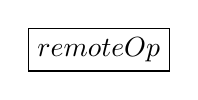
\begin{tikzpicture}
      \node[draw, rectangle, align=center] {$remoteOp$};
    \end{tikzpicture} in the following figures
\end{itemize}

\subsubsection{Causal context}

Associates to a state $S$ a causal context $cc$
\begin{itemize}
  \item Represents all operations known at state $S$
  \item Can use a \emph{version vector} for example as an implementation
\end{itemize}

An example of the lifecycle of such a replicated data structure is shown in figure~\ref{inserts}

\begin{figure}[h]
  \begin{tikzpicture}[
    localOp/.style={->, thick, shorten <=3pt, shorten >=3pt},
    remoteOp/.style={->, dotted, thick, shorten <=3pt, shorten >=3pt},
    trait/.style={fill, rectangle, xscale=0.1},
    medium/.style={scale=0.85}]

    \newcommand{\sOne}{$[(id_1, elt_1)]$}
    \newcommand{\sTwo}{$[(id_1, elt_1), (id_2, elt_2)]$}
    \newcommand{\sThree}{$[(id_1, elt_1), (id_3, elt_3), (id_2, elt_2)]$}

    \node (A) at (0, 0) {node A};
    \node[right=5pt of A] (beginA) {};
    \node[trait, right=of beginA] (S1A) {};
    \drawState{S1A}{above}{$S_1$}{\sOne}{$L_1$}{1/1}
    \node[trait, right=5 of A] (S2A) {};
    \drawState{S2A}{above}{$S_2$}{\sTwo}{$L_2$}{1/1, 2/2}
    \node[right=14 of A] (endA) {};

    \node (B) at (0, -2) {node B};
    \node[right=5pt of B] (beginB) {};
    \node[trait, right=of beginB] (S1B) {};
    \drawState{S1B}{below}{$S_1$}{\sOne}{$L_1$}{1/1}
    \node[trait, right=7 of B] (S2B) {};
    \drawState{S2B}{below}{$S_2$}{\sTwo}{$L_2$}{1/1, 2/2}
    \node[trait, right=6 of S2B] (S3B) {};
    \drawState{S3B}{below}{$S_3$}{\sThree}{$L_3$}{1/1, 2/2, 3/3}
    \node[right=14 of B] (endB) {};

    \draw[->] (beginA) -- (endA);
    \draw[->] (beginB) -- (endB);
    \draw[localOp] (S1A) to[out=-15, in=195] node[below, medium] {$localOp_2=addLocal(1, elt_2)$} (S2A);
    \draw[remoteOp] (S2A) -- node[near start, right, xshift=5pt, medium] {$remoteOp_2=addRemote(id_2, elt_2)$} (S2B);
    \draw[localOp] (S2B) to[out=15, in=165] node[above, medium] {$localOp_3=addLocal(1, elt_3)$} (S3B);

  \end{tikzpicture}
  \caption{Insertion of elements in the replicated sequence}
  \label{inserts}
\end{figure}

\section{$rename$ operations}

\subsection{Motivation}

\begin{itemize}
  \item Identifiers growing over time
  \item Performances of the data structure thus decreasing over time
\end{itemize}

\subsection{$renameLocal$}

\paragraph{Definition}~\\

\begin{itemize}
  \item Add an operation $renameLocal(S) = (S', mapIds, cc_S)$
  \begin{itemize}
    \item Replace each identifier attached to elements of $S$ with new ones
    \item Return a map $mapIds$ of the previous identifiers to the new ones
    \item Also need to return the causal context $cc_S$ of the state $S$
      to indicate on which state has been performed the renaming operation
    \item $view(S) = view(S')$ where $(S', \_, \_) = renameLocal(S)$
  \end{itemize}
\end{itemize}

\paragraph{Algorithm}~\\

The renaming algorithm can be seen here as an algorithm
to distribute evenly a number of values $n$ over an interval $range$.
Such an algorithm is described in \ref{alg:id-rename}:

\begin{algorithm}
  \caption{Identifier renaming algorithm}
  \label{alg:id-rename}
  \begin{algorithmic}
    \Function{renameIdentifier}{$id: Id, index: Int, n: Int$}{$: Id$}
      \State $min \gets MIN$
      \Comment The minimum value of the range used
      \State $max \gets MAX$
      \Comment The maximum value of the range used
      \State $range \gets max - min$
      \State $step \gets range / (n + 1)$
      \State $newPos \gets (index + 1) * step + min$
      \State $id' \gets [<newPos, id.id_{site}, id.clock_{site}>]$
      \State \Return $id'$
    \EndFunction
  \end{algorithmic}
\end{algorithm}

This algorithm can then be used to rename each identifier
for a given state $S$ and generate a mapping between the previous identifiers
and the new ones as shown in \ref{alg:local-rename}:

\begin{algorithm}
  \caption{Local renaming algorithm}
  \label{alg:local-rename}
  \begin{algorithmic}
    \Function{renameLocal}{$S: State$}{$: Map<Id, Id>$}
      \State $mapIds \gets Map()$
      \State $n \gets S.length$
      \ForAll{$(id, elt, index) \in S$}
        \State $id' \gets renameIdentifier(id, index, n)$
        \State $mapIds.set(id, id')$
        \State $id \gets id'$
      \EndFor
      \State \Return $mapIds$
    \EndFunction
  \end{algorithmic}
\end{algorithm}

\paragraph{Limits}~\\

\begin{itemize}
  \item Work only if $n < range$
  \begin{itemize}
    \item Can assume it is generally the case
  \end{itemize}
\end{itemize}

\subsection{$renameRemote$}

\paragraph{Definition}~\\

\begin{itemize}
  \item Add an operation $renameRemote(S, L, mapIds, cc_{S'}) = (S", L")$
  \begin{itemize}
    \item Replace current state $S$ by equivalent state $S"$ and current log $L$ by equivalent log $L"$
    \item Rename all identifiers $id \in S \cap S'$ using $mapIds$
    \item Also have to rename all identifiers $id \in S \cdot id \notin S'$ to preserve the current order of elements
    \item \textbf{Precondition: } $cc_S' \subset cc_S$ ($S$ has seen all the operations seen by $S'$ but may have seen more)
    \item $view(S) = view(S")$ where $(S", \_) = renameRemote(S, L, mapIds, cc_{S'})$
  \end{itemize}
\end{itemize}

\paragraph{Algorithm}~\\

Given an operation $renameRemote(S, L, mapIds, cc_{S'})$,
resulting from the execution of $renameLocal(S')$ on another node,
we have to perform the following algorithm \ref{alg:remote-rename} to apply it:

\begin{algorithm}
  \caption{Remote renaming algorithm}
  \label{alg:remote-rename}
  \begin{algorithmic}
    \Procedure{renameRemote}{$S: State, L: Log, mapIds: Map<Id, Id>, cc_{S'}: StateVector$}
      \State $mapIds' \gets mapIds$
      \ForAll{$remoteOp \in concurrentOps(cc_{S'}, L)$}
      \Comment Get concurrent operations to the renaming
        \State $id \gets remoteOp.id$
        \If{$id \notin mapIds'$}
          \State $prevId \gets prev(id, mapIds)$
          \Comment Get the predecessor of $id$ in $mapIds$
          \State $prevId' \gets mapIds.get(prevId)$
          \State $id' \gets prevId' :: id$
          \Comment Generate the new identifier by concatenating $prevId'$ and $id$
          \State $mapIds'.set(id, id')$
          \State $remoteOp' \gets generateRemoteOp(remoteOp, id')$
          \State $broadcast(remoteOp')$
        \EndIf
      \EndFor
      \ForAll{$(id, elt) \in S$}
        \State $id \gets mapIds'.get(id)$
      \EndFor
    \EndProcedure
  \end{algorithmic}
\end{algorithm}

\paragraph{Limits}~\\

\begin{itemize}
  \item Need a causal delivery of the $rename$ operation
  \begin{itemize}
    \item Actually not necessary
    \item But would have to be able to transform operations from its causal context using $mapIds$
    \item Thus require to keep a reference to $mapIds$
    \item Would be possible to receive an operation which is outdated of several $renaming$
    \item Would have to go through all its transformations
  \end{itemize}
  \item Do not handle concurrent $rename$ operations
  \begin{itemize}
    \item For now, can assume that only one node can perform such operations
  \end{itemize}
  \item $renameRemote$ operation can be bandwidth-consuming (need to send old and new identifiers)
  \begin{itemize}
    \item Can reduce its size but will require more computations
    \item Using the causal context of the operation, we can regenerate original state (replay the log)
    \item Since $renameLocal$ is deterministic, can re-compute $mapIds$ locally
  \end{itemize}
\end{itemize}

\section{Optimisation}

\subsection{Motivation}

As stated previously, the presented mechanism's main flaw is the need to broadcast
$mapIds$, a mapping between the old identifiers to the new ones.
According to the size of the old identifiers, this map may be bandwidth-consuming.

\subsection{Idea}

The algorithm \ref{alg:id-rename} is deterministic. Hence, as long as we provide
to other nodes the required data (identifiers which are renamed,
their index in the data structure, and the number of elements in the data structure),
they will be able to compute the new identifiers.

All these data are actually contained in a sequence composed of the identifiers
which are renamed. We can thus, instead of sending $mapIds$, send such a sequence.

\paragraph{Example}~\\

Instead of broadcasting $(id_1 \rightarrow id_1', id_2 \rightarrow id_2', id_3 \rightarrow id_3')$,
we only need to broadcast to other nodes $[id_1, id_2, id_3]$.\\

We were able to reduce the size of the data to broadcast, but can reduce it further.
Indeed, each identifier is unique. But to refer to one identifier, we do not
need all of its components : we only need two of them, $id.id_{site}$ and $id.clock_{site}$.
Therefore, we are able to reduce again the data to broadcast to a fixed size per element
by discarding every component of the identifier except $id.id_{site}$ and $id.clock_{site}$.

\paragraph{Example}~\\

Instead of broadcasting $[id_1, id_2, id_3]$,
we only need to broadcast to other nodes
$[(id_1.id_{site}, id_1.clock_{site}),
(id_2.id_{site}, id_2.clock_{site}),
(id_3.id_{site}, id_3.clock_{site})]$.

\subsection{Algorithm}

Given such a sequence, we can then recompute $mapIds$
using the following algorithm \ref{alg:recompute-map}:

\begin{algorithm}
  \caption{Map recomputation algorithm}
  \label{alg:recompute-map}
  \begin{algorithmic}
    \Function{recomputeMapIds}{$S: State, L: Log, seq: <Int, Int>[], cc_{S'}: StateVector$}{$: Map<Id, Id>$}
      \State $mapIds \gets Map()$
      \State $n \gets seq.length$
      \State $ids \gets S.map((id, elt) \to id)$
      \Comment Retrieve all identifiers from current state
      \State $ids \gets ids :: L$
      \Comment Retrieve all identifiers from concurrent operations
      \State $~~~~~~~~~~~~~~~~~.filter(remoteOp \to remoteOp.isConcurrent(cc_{S'}))$
      \State $~~~~~~~~~~~~~~~~~.map(remoteOp \to remoteOp.id)$
      \ForAll {$(id_{site}, clock_{site}, index) \in seq$}
        \State $id \gets ids.find(id \to id.id_{site} = id_{site}$ \textbf{and} $id.clock_{site} = clock_{site})$
        \State $id' \gets renameIdentifier(id, index, n)$
        \State $mapIds.set(id, id')$
      \EndFor
      \State \Return $mapIds$
    \EndFunction
  \end{algorithmic}
\end{algorithm}

After recomputing $mapIds$, we can resume the $renaming$ using algorithm \ref{alg:remote-rename}.

\paragraph{Notes:}~\\

\begin{itemize}
  \item Able with this solution to get a fixed size per element in the data broadcasted
    (instead of broadcasting unbounded identifiers).
  \item Need to browse both the state and the concurrent operations
  \begin{itemize}
    \item A renamed identifier may have been deleted concurrently
    \item Thus it won't be in the state
    \item But still need it to properly rename concurrently inserted elements
  \end{itemize}
  \item Cannot factorise this algorithm with the generation of new identifiers
    for concurrent operations
  \begin{itemize}
    \item We need the full $mapIds$ to generate them
  \end{itemize}
\end{itemize}

\section{Discussion}

\begin{itemize}
  \item The size of identifiers from concurrent operations to the $renaming$ operation will increase
  \begin{itemize}
    \item Can argue that they will shrink at next renaming
  \end{itemize}
  \item Can use a mechanism of $epoch$
  \begin{itemize}
    \item Each $rename$ increase the $epoch$ counter
    \item Each operation is labelled with its $epoch$ of generation
    \item Allow us to reject obsoletes operations
  \end{itemize}
  \item Do not require to add other causality information on all operations, only on the $renaming$ one
  \begin{itemize}
    \item The $epoch$ mechanism and the $renaming$'s causal context are sufficient
      to determine the concurrency of operations to the $renaming$ operation
    \item If the $epoch$ is the same as the one before the $renaming$
      and if this operation does not belong to the $renaming$'s causal context,
      this operation is a concurrent one
  \end{itemize}
  \item Performances of the $renaming$ operations depend on the number of elements
    of the data structure, the number of elements of the map
    and the number of concurrent operations
  \item Should be able to adapt the algorithms \ref{alg:local-rename} and \ref{alg:remote-rename}
    to blockwise Identifier-based Sequence \acp{CRDT}
  \begin{itemize}
    \item Here, each element is manipulated one by one (with $add$ and $delete$, but also during search)
    \item In some algorithms like \emph{LogootSplit},
      we actually group elements using blocks
    \item It allows us to:
    \begin{itemize}
      \item Factorise the identifiers of contiguous elements
      \item Reduce the size of the collection by storing
        the blocks instead of elements directly (thus speed up search)
    \end{itemize}
    \item We could adapt the algorithms for these data structures
    \item The $renaming$ operations would thus help us
      to reduce the number of blocks too (could regroup all elements in one new block)
  \end{itemize}
\end{itemize}

\section{Questions}

\begin{itemize}
  \item How to deal with concurrent operations to $renaming$ one when you already applied the $renaming$?
  \begin{itemize}
    \item Can reject it and wait to receive its modified version
    \begin{itemize}
      \item The node which sent us the original version should be able to send us its modified one
      \item But induces some delay
    \end{itemize}
    \item Can use $mapIds$ to compute its transformation
    \begin{itemize}
      \item Need to retrieve it or to compute it again
    \end{itemize}
  \end{itemize}
  \item Which version(s) of the operations to store in the log?
  \begin{itemize}
    \item The original one?
    \item The modified one?
    \item A mix ?
    \item Actually depends on the answer to the previous question
  \end{itemize}
  \item When to trigger the $renaming$?
  \begin{itemize}
    \item According to the size of the longer identifier?
    \item According to the number of elements (in blockwise \acp{CRDT})?
    \begin{itemize}
      \item What would be the thresholds in these cases?
    \end{itemize}
    \item According to the state of the collaboration?
    \begin{itemize}
      \item If the system is idle for example
    \end{itemize}
  \end{itemize}
\end{itemize}

\bibliography{ref-selected}

\end{document}
